\chapter{Data}
\label{chap:data}
In this chapter we introduce the dataset of interest. In Section \ref{section:data:data_exploration} we explore the dataset by extracting key statistics and highlighting interesting characteristics. In order to be able to apply some of the methods of interest that have been mentioned in Chapter \ref{chap:lit_review}, we need to process the data. In general we follow the same steps as has been used by \cite{HartveldKMNPFS18}. We make an explicit mention whenever we deviate from these steps. As a first step, in Section \ref{section:data:data_cleaning}, we explain the data cleaning methods that we apply to the data. Hereafter, in Section \ref{section:data:data_preparation}, we go through the necessary extractions and transformations such that we end with a set of model words per product, to which we can apply variations of LSH. 
\section{Data exploration}
\label{section:data:data_exploration}
The main dataset of interest consists of a list of products and related product information collected by \cite{DamGKNVF16} from four different web shops: \textit{amazon.com}, \textit{newegg.com}, \textit{bestbuy.com}, and \textit{thenerds.net}s. The dataset amounts to a total of 1624 products. We give an overview of the number of products per shop in Table \ref{table:no_products_per_shop}. All products that have been collected from the same Web shop are verified to relate to different real-world entities. In other words, there are no duplicates to be found in such a set of products. On the other hand, there might be products listed in distinct Web shops, that do refer to the same real-world entity. Conclusively, we are dealing with a Clean-Clean ER problem.
\begin{table}
    \centering
    \caption{List of shops and number of products per shop}
    \begin{tabular}{ |c|c| } 
     \hline
     Shop & Number of products \\ 
     \hline
     bestbuy.com & 773  \\ 
     \hline
     newegg.com & 668  \\ 
     \hline
     amazon.com &  163 \\ 
     \hline
     thenerds.net & 20  \\ 
     \hline
    \end{tabular}
\label{table:no_products_per_shop}
\end{table}

Each product comes with a product title, model id, retrieval-url, and a list of attributes in the form of key-value pairs, where the key represents the name of the attribute and the value the specific value. The model id is the key that we can use to determine to which real-world entity a product is related. In practice, this model id is generally not available, but we use the information on model ids in our set-up to verify that the methods correctly identify duplicates. If we apply a group by operation on the model id key and count the number of products in each group, we obtain the number of duplicates per model id.  We find that there are $300$ regular duplicates, where products related to the same real-world entity occur in two different Web shops, $25$ triple duplicates, where products related to the same real-world entity occur in three different Web shops, and $4$ occurences of quadadruple duplicates, where products related to the same real-world entity occur in all four Web shops. It logically follows that we are left with $1624 - (300 * 2 + 25 * 3 + 4 * 4) = 933$ products that are uniquely identified by a model id. A comprehensive overview of these statistics can be found in table \ref{table:no_duplicates_occurences}.

\begin{table}
    \centering
    \caption{Type of duplicates and frequency of occurence}
    \begin{tabular}{ |c|c| } 
     \hline
     Number of duplicates & Occurences \\ 
     \hline
     - (no duplicates) & 933 \\
     \hline
     2 & 300  \\ 
     \hline
     3 & 25  \\ 
     \hline
     4 & 4  \\ 
     \hline
    \end{tabular}
    
    \label{table:no_duplicates_occurences}
\end{table}

The feature lists of products do not follow a pre-defined structure. Between the Web shops, but also within a single Web shop we find a large variation in the number and type of keys available in the feature lists of the products (see Table \ref{table:keys}). In general we can conclude that \textit{amazon.com} provides less extensive information than other webshops, while \textit{thenerds.net} can be placed on the other end of the spectrum, including on average more than $55$ keys per product and $121$ unique keys over all products. This last fact is even more impressive considering that there are only $20$ products from \textit{thenerds.net} in the dataset. The fact that the schema of our inputs differs so vastly not only on a between shop basis, but also on a within shop basis, highlights the need for schema-agnostic methods that can achieve high-quality, efficient deduplication.
\begin{table}
    \centering
    \caption{Statistics on the use of keys in the feature list of products on a per-shop basis.}
    \begin{tabular}{ |c|c|c|c|c| } 
     \hline
     Shop & No. unique keys & Avg. no. keys & Min. no. keys & Max. no. keys \\ 
     \hline
     bestbuy.com & 129 & 37.05 &  4 & 61 \\
     \hline
     newegg.com & 88 & 22.59 & 1 & 46  \\ 
     \hline
     amazon.com & 31 & 10.17 & 5 & 17  \\ 
     \hline
     thenerds.net & 121 & 56.05 & 19 & 65    \\ 
     \hline
    \end{tabular}
    \label{table:keys}
\end{table}

\section{Data cleaning}
\label{section:data:data_cleaning}
The driving factor for the methods of deduplication in this research is the identification of matching model words in distinct product listings. In some cases different variations of those model words exist, while they actually refer to the exact same real-world entity. This is mainly due to different textual representations of measures, such as ``"'', ``inch'', and ``in'', or ``Hz'', ``HZ'', and ``hz''. For each type of measure, we search through the title and key-value pairs of each product, replacing the different variations by the \textit{normalized} value. The \textit{normalized} values and alternative representations are listed in table \ref{table:data_cleaning}.
\begin{table}
    \centering
    \caption{Normalized values and alternative representations.}
    \begin{tabular}{ |c|c| } 
     \hline
     Normalized value & Alternative representations in data\\ 
     \hline
     inch & \{``"'', `` inch'', ``inches'', ``Inch'', ``-inch'', ``-Inch'' \} \\
     \hline
     lb & \{``lb.'', ``lbs.'', ``pounds'', `` pounds'', `` lbs'', `` lb'' \} \\ 
     \hline
     hz & \{``HZ'', ``Hz'', ``Hertz'', ``hertz'', `` hz'', ``-hz'' \} \\ 
     \hline
    \end{tabular}
    
    \label{table:data_cleaning}
\end{table}

\section{Data preparation}
\label{section:data:data_preparation}
In order to determine whether two products are the same, information on the brand is very helpful. By definition, two televisions from two different brands cannot refer to the same real-world entity, which greatly reduces the number of necessary comparisons. We downloaded a list of television brands from Wikipedia\footnote{list of television brands can be found on https://en.wikipedia.org/wiki/List\_of\_television\_manufacturers}. This list is available in the thesis' GitHub repository. We first check if any of the brand names is contained in the title. If no brand is found in the title, the search is continued in the values of the key-value pairs of the products. If this search is fruitless as well, the brand name 'Unknown' is assigned to the product. 
\begin{table}
    \centering
    \caption{Extracted brands and the number of products that is assigned to each brand.}
    \begin{tabular}{ |c|c|c|c|c|c|c|c| } 
     \hline
     Brand name & Occurences & Brand name & Occurences & Brand name & Occurences & Brand name & Occurences\\ 
     \hline
    %  Affinity & 2 & Insignia & 39 & Pyle & 3 & Supersonic & 9\\
    %  \hline
    %  Coby & 29 & JVC & 15 & RCA & 24 & TCL & 11\\ 
    %  \hline
    %  Contex & 4 & Magnavox & 8 & SEI & 6 & Toshiba & 120\\ 
    %  \hline
    %  Craig & 1 & Mitsubishi & 3 & Samsung & 417 & Unknown & 11\\ 
    %  \hline
    %  Electron & 3 & NEC & 15 & Sansui & 20 & Upstar & 2 \\ 
    %  \hline
    %  Elite & 2 & Naxa & 5 & Sanyo & 20 & Viewsonic & 10\\ 
    %  \hline
    %  Haier & 4 & One & 1 & Sceptre & 7 & Vizio & 95\\ 
    %  \hline
    %  Hannspree & 4 & Panasonic & 117 & Sharp & 87 & Westinghouse & 3\\ 
    %  \hline
    %  Hisense & 4 & Philips & 39 & Sony & 86 & Dynex & 18\\ 
    %  \hline
    %  Ice & 4 & Proscan & 6 & SunBriteTV & 14 & LG & 335 \\ 
    %  \hline

    Affinity &      2 &         Ice &      1 &  Philips &     39 &          Sony &     86 \\ \hline
    Coby &     29 &    Insignia &     39 &  ProScan &      6 &    SunBriteTV &     14 \\ \hline
    Contex &      4 &         JVC &     15 &     Pyle &      3 &    Supersonic &      9 \\ \hline
    Craig &      1 &          LG &    335 &      RCA &     24 &           TCL &     11 \\ \hline
    Dynex &     18 &    Magnavox &      8 &      SEI &      6 &           Tec &      1 \\ \hline
    Electron &      3 &  Mitsubishi &      3 &  Samsung &    417 &       Toshiba &    120 \\ \hline
    Elite &      2 &         NEC &     15 &   Sansui &     20 &        Upstar &      2 \\ \hline
    Haier &     24 &        Naxa &      5 &    Sanyo &     10 &     Viewsonic &     10 \\ \hline
    Hannspree &      4 &         One &      1 &  Sceptre &      7 &         Vizio &     95 \\ \hline
    Hisense &      5 &   Panasonic &    117 &    Sharp &     87 &  Westinghouse &     15 \\ \hline
    \end{tabular}
    \label{table:brands_in_data}
\end{table}

After the extraction of brands, it is time to extract the model words related to each product. Following the approach put forward by \cite{HartveldKMNPFS18}, we extract model words from the title and the attribute values. A model word in the title is defined as a sequence of both numeric and alphabetic/punctuation characters, such as ``46inch'' or ``5lbs''. Such words can be captured by the following regular expression:

\begin{center}
    $\text{ModelWord}_{\text{title}}$ = \verb !([a-zA-Z0-9]*(([0-9]+[^0-9, ]+)|([^0-9, ]+[0-9]+))[a-zA-Z0-9]*)!
\end{center}
The subpattern \verb!([0-9]+[^0-9, ]+)|([^0-9, ]+[0-9]+)! ensures that the word contains a combination of numeric (\verb![0-9]+!) and non-numeric (\verb![^0-9, ]+!) tokens, while the addition of the subpattern \verb![a-zA-Z0-9]*!, matching all alphanumeric tokens, at the start and end of the regex pattern, ensures that words that contain additional alphanumeric charactes at the start or end are also included in the list of model words.

For the model words in the attributes we use the extended definition of a model word, as proposed by \cite{HartveldKMNPFS18}. As these attributes tend to include more detailed information on the technical charateristics of the television, we define a model word as a decimal number with an optional alphabetic part. The following regex expression aims to identify such words.

\begin{center}
$\text{ModelWord}_{\text{attributes}}$ = \verb !(^\d+(\.\d+)?[a-zA-Z]+$|^\d+(\.\d+)?$)!
\end{center}

The subpattern \verb!^\d+(\.\d+)?! identifies decimal numbers. In the first part of the regex this subpattern is paired with the subpattern \verb![a-zA-Z]+!. This combination identifies decimal numbers with a non-numeric part, such as $46.0$inch. The second part solely uses \verb!^\d+(\.\d+)?! for identification of decimal numbers. 

We proceed by deleting the non-numerical part of the value-based model words. This ensures that model words that have the same value for an attribute and a different representation of that attribute still contribute to the similarity of products.

For each entity in our dataset, we place the extracted model words from the title and attribute values in a set of model words per entity. It might be that the model id of the product is among the extracted model words. These are deleted from the set of model words, since we want the results of our application to be applicable to problems where the model id of a product is unknown. The resulting sets of model words serve as input for the LSH applications, on which we expand further in Chapter \ref{chap:methodology}. 

Running the aforementioned procedure, we obtain on average $10.38$ model words per entity. This means that for the average entity in our dataset FSS is a more efficient sketching procedure than MinHash provided that the sketch length $n \leq e^{10.38} \approx 32208$. This constraint is easily met in all practical LSH applications. 

Using the obtained model words, we can calculate the actual Jaccard similarities of the $399$ true pairwise duplicates in the dataset. The average actual Jaccard similarity turns out to be $0.3192$. How does this compare to the Jaccard similarity of the average pair in the dataset? To answer this question, we randomly sample $399$ pairs from the dataset and calculate the Jaccard similarity of each pair. The average Jaccard similarity of these pairs comes down to $0.1227$. In Figure \ref{fig:jaccard_true_dup_ran_pair} we compare the Jaccard similarity of the true pairwise duplicates with the Jaccard similarity of the selection of random pairs.

\begin{figure}
    \centering
    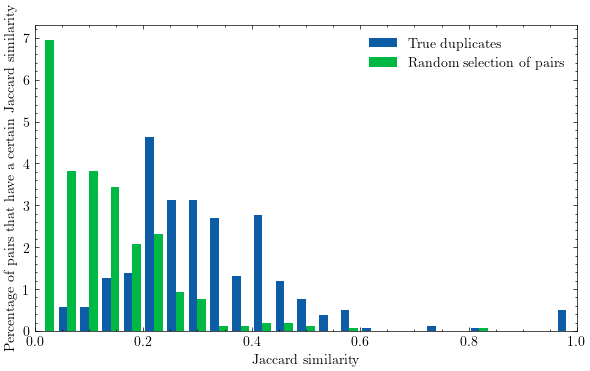
\includegraphics[width=0.75\textwidth]{jaccard_true_dup_random_pairs.png}
    \caption[Jaccard similarity of true duplicates compared to selection of random pairs]{\textbf{Jaccard similarity of true duplicates compared to selection of random pairs}.}
    \label{fig:jaccard_true_dup_ran_pair}
\end{figure}
